\subsection{Example \#1 -- the IQ score}
We get a random sample of 200 people and give them an IQ test. From this sample, we want to infer the true distribution in the entire population.

Suppose that the IQ in the general population has a normal distribution with mean=100 and  standard deviation =15, and from this population we draw 200 people, and calculate the sample mean and standard deviation:

\begin{knitrout}
\definecolor{shadecolor}{rgb}{0.969, 0.969, 0.969}\color{fgcolor}\begin{kframe}
\begin{alltt}
\hlkwd{set.seed}\hlstd{(}\hlnum{95473}\hlstd{)}
\hlstd{n} \hlkwb{<-} \hlnum{200}
\hlstd{samp} \hlkwb{<-} \hlkwd{rnorm}\hlstd{(n,} \hlnum{100}\hlstd{,} \hlnum{15}\hlstd{)}
\hlkwd{cat}\hlstd{(}\hlstr{"Mean="}\hlstd{,}\hlkwd{mean}\hlstd{(samp),} \hlstr{", SD="}\hlstd{,}\hlkwd{sd}\hlstd{(samp),}\hlstr{"\textbackslash{}n"}\hlstd{)}
\end{alltt}
\begin{verbatim}
## Mean= 99.38613 , SD= 15.55667
\end{verbatim}
\end{kframe}
\end{knitrout}

We notice that the sample mean is 99.4 and the sample standard deviation is 15.6. Both are very close to the true values. 

Let's pretend that just like in real life, we don't know the true distribution, so we have to check if the mathematical model we chose (normal distribution) is appropriate for the data from the finite sample. When it is assumed that the data come from a normal distribution, we can use the \code{qqnorm} function to check if the assumption is reasonable:

\begin{knitrout}
\definecolor{shadecolor}{rgb}{0.969, 0.969, 0.969}\color{fgcolor}\begin{kframe}
\begin{alltt}
\hlkwd{qqnorm}\hlstd{(samp,} \hlkwc{cex}\hlstd{=}\hlnum{0.7}\hlstd{,} \hlkwc{pch}\hlstd{=}\hlnum{18}\hlstd{,} \hlkwc{col}\hlstd{=}\hlstr{"purple"}\hlstd{)}
\hlkwd{abline}\hlstd{(}\hlnum{100}\hlstd{,}\hlnum{15}\hlstd{,}\hlkwc{col}\hlstd{=}\hlstr{"orange"}\hlstd{,} \hlkwc{lwd}\hlstd{=}\hlnum{3}\hlstd{)}
\end{alltt}
\end{kframe}\begin{figure}

{\centering 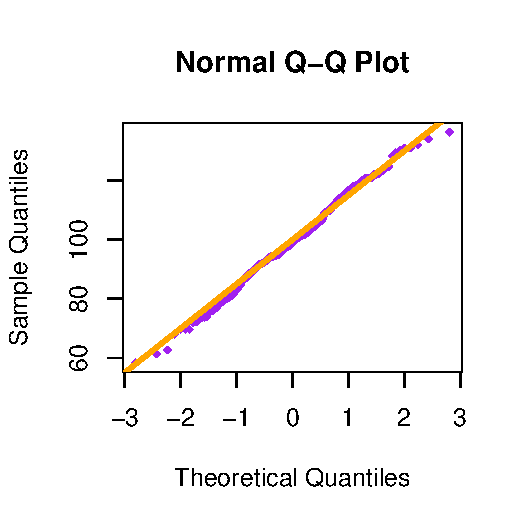
\includegraphics[width=\maxwidth]{figure/intro-lln1-1-1} 

}

\caption[Q-Q plot for the simulated IQ scores]{Q-Q plot for the simulated IQ scores.}\label{fig:intro-lln1-1}
\end{figure}

\end{knitrout}

The points in the Q-Q plot lie very close to a straight line, indicating that the sample  was  likely drawn from a normal distribution (because we generated it this way, this is not surprising. However, when we get a random sample and we do not know the true distribution, this plot is useful to check whether our mathematical model is reasonable.)

To understand what the LLN, let's obtain samples of varying sizes and see what happens to the sample mean as we increase $n$. 

\begin{knitrout}
\definecolor{shadecolor}{rgb}{0.969, 0.969, 0.969}\color{fgcolor}\begin{kframe}
\begin{alltt}
\hlkwd{set.seed}\hlstd{(}\hlnum{95473}\hlstd{)}
\hlstd{ns} \hlkwb{<-} \hlkwd{seq}\hlstd{(}\hlnum{10}\hlstd{,} \hlnum{2000}\hlstd{,} \hlkwc{by}\hlstd{=}\hlnum{10}\hlstd{)}
\hlstd{L} \hlkwb{<-} \hlkwd{length}\hlstd{(ns)}
\hlstd{allMeans} \hlkwb{<-} \hlkwd{rep}\hlstd{(}\hlnum{0}\hlstd{, L)}
\hlkwa{for} \hlstd{(i} \hlkwa{in} \hlnum{1}\hlopt{:}\hlstd{L) \{}
  \hlstd{samp} \hlkwb{<-} \hlkwd{rnorm}\hlstd{(ns[i],} \hlnum{100}\hlstd{,} \hlnum{15}\hlstd{)}
  \hlstd{allMeans[i]} \hlkwb{<-} \hlkwd{mean}\hlstd{(samp)}
\hlstd{\}}
\hlkwd{plot}\hlstd{(ns, allMeans,} \hlkwc{pch}\hlstd{=}\hlnum{19}\hlstd{,} \hlkwc{cex}\hlstd{=}\hlnum{0.5}\hlstd{,} \hlkwc{col}\hlstd{=}\hlnum{3}\hlstd{,} \hlkwc{axes}\hlstd{=}\hlnum{FALSE}\hlstd{)}
\hlkwd{axis}\hlstd{(}\hlnum{1}\hlstd{);} \hlkwd{axis}\hlstd{(}\hlnum{2}\hlstd{)}
\hlkwd{abline}\hlstd{(}\hlkwc{h}\hlstd{=}\hlnum{100}\hlstd{,} \hlkwc{lwd}\hlstd{=}\hlnum{3}\hlstd{,}\hlkwc{col}\hlstd{=}\hlnum{2}\hlstd{)}
\end{alltt}
\end{kframe}\begin{figure}

{\centering 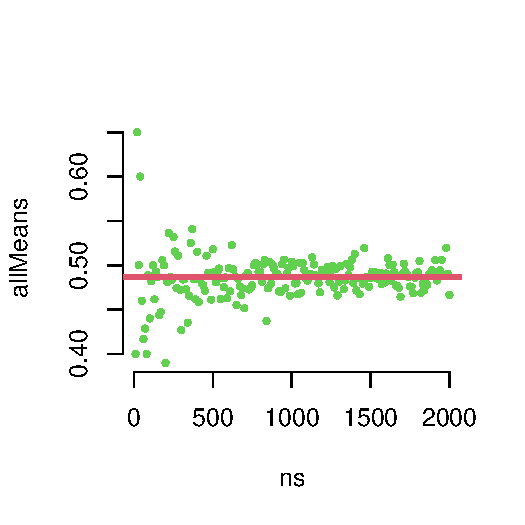
\includegraphics[width=\maxwidth]{figure/intro-lln1-2-1} 

}

\caption[Q-Q plot for the simulated IQ scores]{Q-Q plot for the simulated IQ scores.}\label{fig:intro-lln1-2}
\end{figure}

\end{knitrout}

We see that as $n$ increases, the sample mean gets closer to the true mean (100).

